\documentclass{assignment}
\ProjectInfos{高等热力学与统计物理}{PHYS2110}{2020-2021学年第二学期}{期末考试}{截止时间:2021. 6. 16(周三)12:00}{陈稼霖}{45875852}

\begin{document}
\begin{itemize}
    \item 通用符号:$T=$ 温度,$P=$ 压强,$V=$ 体积,$N=$ 粒子数,$\rho=$ 数密度,$\mu=$ 化学势,$k=$ Boltzmann 常数,$\hbar=$ Plank 常数.
    \item 热力学极限:
    \[
        N\rightarrow\infty\quad V\rightarrow\infty\quad\rho=\frac{N}{V}\neq 0\text{且有限}.
    \]
\end{itemize}
\begin{prob}
    某一磁性物质对外界所做的微功为
    \[
        \delta W=-H\mathrm{d}M
    \]
    其中 $H$ 和 $M$ 为磁场强度和磁化强度. 体积固定且设为 $1$.\\
    如果 $H$, $M$ 和 温度 $T$ 的关系为
    \[
        M=\frac{aH}{T-T_c}
    \]
    $a$, $T_c$ 为常数且 $T>T_c$.
    \begin{itemize}
        \item[1)] 证明该物质的内能由下式给出:(10 分)
        \[
            U(T,M)=U(T,0)-\frac{M^2T_c}{2a}.
        \]
        \item[2)] 求该物质在 $H$ 固定条件下的热容量,$C_H(T,M)$.(10 分)
    \end{itemize}
\end{prob}
\begin{sol}
    \begin{itemize}
        \item[1)] 由热力学第一定律的微分形式
        \begin{align}
            \mathrm{d}U=\delta Q-\delta W=T\,\mathrm{d}S+H\,\mathrm{d}M.
        \end{align}
        以及 Helmholtz 自由能的定义
        \begin{align}
            F=U-TS,
        \end{align}
        可得 Helmholtz 自由能的微分为
        \begin{align}
            \mathrm{d}F=-S\,\mathrm{d}T+H\,\mathrm{d}M.
        \end{align}
        由上式可得
        \begin{align}
            S=&-\left(\frac{\partial F}{\partial T}\right)_M,\\
            H=&\left(\frac{\partial F}{\partial M}\right)_T.
        \end{align}
        以上两式分别关于磁化强度 $M$ 和 温度 $T$ 求导可得
        \begin{align}
            \label{1-dS/dM=-dH/dT}
            \left(\frac{\partial S}{\partial M}\right)_T=-\frac{\partial^2F}{\partial M\partial T}=-\left(\frac{\partial H}{\partial T}\right)_M.
        \end{align}

        在给定温度下,磁性物质的内能关于磁化强度 $M$ 的偏导为
        \begin{align}
            \left(\frac{\partial U}{\partial M}\right)_T=T\left(\frac{\partial S}{\partial M}\right)_T+H.
        \end{align}
        将式 \eqref{1-dS/dM=-dH/dT} 以及 $H$, $M$ 和 $T$ 的关系 $M=\frac{aH}{T-T_c}$,代入上式可得
        \begin{align}
            \label{1-dU/dM}
            \left(\frac{\partial U}{\partial M}\right)_T=-T\left(\frac{\partial H}{\partial T}\right)_M+H=-\frac{TM}{a}+\frac{(T-T_c)M}{a}=-\frac{T_cM}{a}.
        \end{align}
        因此,
        \begin{align}
            U(T,M)=U(T,0)+\int_0^M\left(\frac{\partial U}{\partial M}\right)_T\,\mathrm{d}M=U(T,0)-\int_0^M\frac{T_cM'}{a}\,\mathrm{d}M'=U(T,0)-\frac{T_cM^2}{2a}.
        \end{align}
        \item[2)] 该物质在 $H$ 固定条件下的热容量为
        \begin{align}
            C_H(T,M)=&\lim_{\Delta T\rightarrow 0}\left(\frac{\Delta Q}{\Delta T}\right)_H=\lim_{\Delta T\rightarrow 0}\left(\frac{\Delta U-H\,\mathrm{d}M}{\Delta T}\right)_H=\frac{\mathrm{d}U(T,M=0)}{\mathrm{d}T}-\frac{T_cM}{a}\left(\frac{\partial M}{\partial T}\right)_H-H\left(\frac{\partial M}{\partial T}\right)_H\\
            =&\frac{\mathrm{d}U(T,M=0)}{\mathrm{d}T}+\left(\frac{T_cM}{a}+H\right)\frac{aH}{(T-T_c)^2}=\frac{\mathrm{d}U(T,M=0)}{\mathrm{d}T}+\frac{TM^2}{a(T-T_c)}.
        \end{align}
        % 一方面,由热力学第一定律以及该物质在 $H$ 固定下的热容量的定义 $C_M(T,M)=\left(\frac{\partial U}{\partial T}\right)_M$,
        % \begin{align}
        %     T\,\mathrm{d}S=\mathrm{d}U-H\,\mathrm{d}M=\left(\frac{\partial U}{\partial T}\right)_M\,\mathrm{d}T+\left(\frac{\partial U}{\partial M}\right)_T\,\mathrm{d}M-H\,\mathrm{d}M=C_M\,\mathrm{d}T+\left(\frac{\partial U}{\partial M}\right)_T\,\mathrm{d}M-H\,\mathrm{d}M.
        % \end{align}
        % 将式 \eqref{1-dU/dM} 代入上式可得
        % \begin{align}
        %     \label{1-TdS-1}
        %     T\,\mathrm{d}S=C_M\,\mathrm{d}T-T\left(\frac{\partial H}{\partial T}\right)_M\,\mathrm{d}M.
        % \end{align}
        % 另一方面,该物质的 Gibbs 势为
        % \begin{align}
        %     G=U-TS-HM.
        % \end{align}
        % 从而 Gibbs 势的微分为
        % \begin{align}
        %     \mathrm{d}G=-S\,\mathrm{d}T-M\,\mathrm{d}H.
        % \end{align}
        % 由上式得
        % \begin{align}
        %     S=&-\left(\frac{\partial G}{\partial T}\right)_H,\\
        %     M=&-\left(\frac{\partial G}{\partial H}\right)_T.
        % \end{align}
        % 以上两式分别关于磁场强度 $H$ 和熵 $S$ 求偏导可得
        % \begin{align}
        %     \label{1-dT/dH=-dM/dS}
        %     \left(\frac{\partial S}{\partial H}\right)_T=\frac{\partial^2\mathcal{H}}{\partial S\partial H}=-\left(\frac{\partial M}{\partial T}\right)_H.
        % \end{align}
        % 磁性物质的焓定义为
        % \begin{align}
        %     \mathcal{H}=U-HM,
        % \end{align}
        % 焓的微分为
        % \begin{align}
        %     \label{1-dH}
        %     \mathrm{d}\mathcal{H}=T\,\mathrm{d}S-M\,\mathrm{d}H,
        % \end{align}
        % 焓 $\mathcal{H}$ 关于磁场强度 $H$ 的偏导为
        % \begin{align}
        %     \left(\frac{\partial\mathcal{H}}{\partial H}\right)_T=T\left(\frac{\partial S}{\partial H}\right)_T-M.
        % \end{align}
        % 将式 \eqref{1-dT/dH=-dM/dS} 代入上式可得
        % \begin{align}
        %     \label{1-dH/dH}
        %     \left(\frac{\partial\mathcal{H}}{\partial H}\right)_T=-T\left(\frac{\partial M}{\partial T}\right)_H-M.
        % \end{align}
        % 该物质在 $H$ 固定条件下的热容量 $C_H(T,M)=\left(\frac{\partial U}{\partial T}\right)_H-H\left(\frac{\partial M}{\partial T}\right)_H=\left(\frac{\partial\mathcal{H}}{\partial T}\right)_H$,由式 \eqref{1-dH}
        % \begin{align}
        %     T\,\mathrm{d}S=\mathrm{d}\mathcal{H}+M\,\mathrm{d}H=\left(\frac{\partial\mathcal{H}}{\partial T}\right)_H\,\mathrm{d}T+\left(\frac{\partial\mathcal{H}}{\partial H}\right)_T\,\mathrm{d}H+M\,\mathrm{d}H=C_H\,\mathrm{d}T+\left(\frac{\partial\mathcal{H}}{\partial H}\right)_T\,\mathrm{d}H+M\,\mathrm{d}H.
        % \end{align}
        % 将式 \eqref{1-dH/dH} 以及 $H$, $M$ 和 $T$ 的关系 $M=\frac{aH}{T-T_c}$,代入上式可得
        % \begin{align}
        %     \label{1-TdS-2}
        %     T\,\mathrm{d}S=C_H\,\mathrm{d}T-T\left(\frac{\partial M}{\partial T}\right)_H\,\mathrm{d}H.
        % \end{align}

        % 式 \eqref{1-TdS-1} 和 \eqref{1-TdS-2} 联立消去 $T\,\mathrm{d}S$ 得
        % \begin{gather}
        %     (C_H-C_M)\,\mathrm{d}T=T\left[\left(\frac{\partial M}{\partial T}\right)_H\,\mathrm{d}H+\left(\frac{\partial H}{\partial T}\right)_M\,\mathrm{d}M\right],\\
        %     \label{1-dT-1}
        %     \Longrightarrow\mathrm{d}T=\frac{T}{C_H-C_M}\left[\left(\frac{\partial H}{\partial T}\right)_M\,\mathrm{d}M+\left(\frac{\partial M}{\partial T}\right)_H\,\mathrm{d}H\right]
        % \end{gather}
        % 由状态方程得
        % \begin{align}
        %     \label{1-dT-2}
        %     \mathrm{d}T=\left(\frac{\partial T}{\partial M}\right)_H\,\mathrm{d}M+\left(\frac{\partial T}{\partial H}\right)_M\mathrm{d}H
        % \end{align}
        % 比较上面两式(\eqref{1-dT-1} 和 \eqref{1-dT-2})可得
        % \begin{align}
        %     \frac{T}{C_H-C_M}\left(\frac{\partial H}{\partial T}\right)_M=&\left(\frac{\partial T}{\partial M}\right)_H,\\
        %     \frac{T}{C_H-C_M}\left(\frac{\partial M}{\partial T}\right)_H=&\left(\frac{\partial T}{\partial H}\right)_M,
        % \end{align}
        % \begin{align}
        %     \label{1-CH-CM}
        %     \Longrightarrow C_H-C_M=\frac{T\left(\frac{\partial H}{\partial T}\right)_M}{\left(\frac{\partial T}{\partial M}\right)_H}.
        % \end{align}

        % 接下来考虑绝热过程,令式 \eqref{1-TdS-1} 和 \eqref{1-TdS-2} 中的 $\mathrm{d}S=0$,有
        % \begin{align}
        %     C_M=&T\left(\frac{\partial H}{\partial T}\right)_M\left(\frac{\partial M}{\partial T}\right)_S,\\
        %     C_H=&T\left(\frac{\partial M}{\partial T}\right)_H\left(\frac{\partial H}{\partial T}\right)_S.
        % \end{align}
        % 上面两式相除可得
        % \begin{align}
        %     \label{1-CH/CM}
        %     \frac{C_H}{C_M}=\frac{\left(\frac{\partial M}{\partial T}\right)_H\left(\frac{\partial H}{\partial T}\right)_S}{\left(\frac{\partial H}{\partial T}\right)_M\left(\frac{\partial M}{\partial T}\right)_S}=-\frac{\left(\frac{\partial M}{\partial H}\right)_T}{\left(\frac{\partial M}{\partial H}\right)_S}=
        % \end{align}
        % 联立式 \eqref{1-CH-CM} 和 \eqref{1-CH/CM} 可得
        % \begin{align}
        %     C_H=-\frac{T\left[\left(\frac{\partial M}{\partial T}\right)_H\right]^2}{\left(\frac{\partial M}{\partial H}\right)_T-\left(\frac{\partial M}{\partial H}\right)_S}
        % \end{align}
        % 其中根据 $H$, $M$ 和 $T$ 的关系 $M=\frac{aH}{T-T_c}$,
        % \begin{align}
        %     \left(\frac{\partial M}{\partial T}\right)_H=&-\frac{aH}{(T-T_c)^2},\\
        %     \left(\frac{\partial M}{\partial H}\right)_T=&\frac{a}{T-T_c}.
        % \end{align}
        % 在绝热磁化中,
    \end{itemize}
\end{sol}
\clearpage

\begin{prob}
    一温度为 $T$ 的圆柱形容器被一活塞隔成两部分. 每部分放置一种非相对论 Fermi 气体. 活塞可以自由移动. 两种 Fermi 气体的分子质量相同,但自旋不同,分别为 $j_1$ 和 $j_2$. 求 $T=0$ 和 $T\rightarrow\infty$ 条件下两种 Fermi 气体分子数密度的比值.(20 分)
    \begin{figure}[h]
        \centering
        
\includegraphics[width=.5\columnwidth]{P2.png}
    \end{figure}
\end{prob}
\begin{sol}
    非简并情况下,非相对论 Fermi 气体的状态方程为
    \begin{align}
        \frac{P}{kT}=\frac{\omega}{\lambda^3}\left(z-\frac{z^2}{2^{5/2}}+\cdots\right).
    \end{align}
    粒子数密度为
    \begin{align}
        \rho=\frac{\omega}{\lambda^3}\left(z-\frac{z^2}{2^{3/2}}+\cdots\right).
    \end{align}
    其中热波长 $\lambda=\sqrt{\frac{2\pi}{mkT}}\hbar$,易逸度 $z=e^{\beta\mu}$. 在 $T\rightarrow\infty$ 条件下,$z\ll 1$,以上两式联立解得
    \begin{align}
        \frac{P}{kT}=\rho\left(1+\frac{1}{2^{5/2}}\frac{\rho\lambda^3}{\omega}+\cdots\right).
    \end{align}
    容器温度给定,故两部分气体温度相等,$T_1=T_2$;活塞可以自由移动,故两部分气体压强相等,$P_1=P_2$. 故\uline{在 $T\rightarrow\infty$ 条件下},两部分气体的分子数密度为
    \begin{align}
        \boxed{\frac{\rho_1}{\rho_2}=1.}
    \end{align}

    非相对论气体的态密度为
    \begin{align}
        D(\varepsilon)=\frac{(2j+1)m^{3/2}\varepsilon^{1/2}}{\sqrt{2}\pi^2\hbar^3}.
    \end{align}
    分子数密度为
    \begin{gather}
        \label{2-rho-epsilonF}
        \rho=\frac{N}{V}=\int_0^{\varepsilon_F}\mathrm{d}\varepsilon\,D(\varepsilon)=\int_0^{\varepsilon_F}\mathrm{d}\varepsilon\,\frac{(2j+1)m^{3/2}\varepsilon^{1/2}}{\sqrt{2}\pi^2\hbar^3}=\frac{2}{3}\frac{(2j+1)m^{3/2}\varepsilon_F^{3/2}}{\sqrt{2}\pi^2\hbar^3},\\
        \Longrightarrow\varepsilon_F=\left[\frac{3}{\sqrt{2}}\frac{\pi^2\hbar^3}{(2j+1)m^{3/2}}\frac{N}{V}\right]^{2/3}.
    \end{gather}
    在 $T=0$ 下,非相对论 Fermi 气体的内能为
    \begin{align}
        U=V\int_0^{\varepsilon_F}\mathrm{d}\varepsilon\,D(\varepsilon)\varepsilon=V\frac{2}{5}\frac{(2j+1)m^{3/2}\varepsilon_F^{5/2}}{\sqrt{2}\pi^2\hbar^3}.
    \end{align}
    因此
    \begin{align}
        U\propto V^{-2/3}.
    \end{align}
    压强为
    \begin{align}
        P=-\frac{\partial U}{\partial V}=\frac{2}{3}\frac{U}{V}=\frac{4}{15}\frac{(2j+1)m^{3/2}\varepsilon_F^{5/2}}{\sqrt{2}\pi^2\hbar^3}.
    \end{align}
    活塞可以自由移动,故两部分气体压强相等,$P_1=P_2$,即
    \begin{gather}
        \frac{4}{15}\frac{(2j_1+1)m^{3/2}\varepsilon_{F,1}^{5/2}}{\sqrt{2}\pi^2\hbar^3}=\frac{4}{15}\frac{(2j_2+1)m^{3/2}\varepsilon_{F,2}^{5/2}}{\sqrt{2}\pi^2\hbar^3},\\
        \Longrightarrow\frac{\varepsilon_{F,1}}{\varepsilon_{F,2}}=\left(\frac{2j_1+1}{2j_2+1}\right)^{-2/5}.
    \end{gather}
    将上式代入式 \eqref{2-rho-epsilonF} 中可得在 \uline{$T=0$ 条件下},两部分气体的分子数密度比值为
    \begin{align}
        \boxed{\frac{\rho_1}{\rho_2}=\frac{2j_1+1}{2j_2+1}\left(\frac{\varepsilon_{F,1}}{\varepsilon_{F,2}}\right)^{3/2}=\left(\frac{2j_1+1}{2j_2+1}\right)^{2/5}.}
    \end{align}

    综上,在 $T=0$ 和 $T\rightarrow\infty$ 条件下两种 Fermi 气体分子数密度的比值为
    \begin{align}
        \boxed{\frac{\rho_1}{\rho_2}=\left\{\begin{array}{ll}
            \left(\frac{2j_1+1}{2j_2+1}\right)^{2/5},&T=0.\\
            1,&T\rightarrow\infty.
        \end{array}\right.}
    \end{align}
\end{sol}
\clearpage

\begin{prob}
    考虑一低密度的经典单原子非理想气体,原子之间的相互作用势能为
    \[
        u(r)=\left\{\begin{array}{ll}
            \infty,&r\leq a\\
            -g,&a<r<b\\
            0,&r\geq b
        \end{array}\right.
    \]
    \begin{itemize}
        \item[1)] 求精确到 $\rho^2$ 的状态方程,即把 $P/kT$ 展开到 $\rho^2$.(10 分)
        \item[2)] 求该气体的化学势对理想气体化学势的领头阶修正.(5 分)
        \item[3)] 求该气体的熵和内能对理想气体熵和内能的领头阶修正.(5 分)
    \end{itemize}
\end{prob}
\begin{sol}
    \begin{itemize}
        \item[1)] 根据原子之间的相互作用势能,有
        \begin{align}
            f_{ij}(r)=e^{-\beta u_{ij}(r)}-1=\left\{\begin{array}{ll}
                -1,&r\leq a,\\
                e^{\beta g}-1,&a<r<b,\\
                0,&r\geq b.
            \end{array}\right.
        \end{align}
        利用 Mayer 第二定理对 $\frac{P}{kT}$ 按 $\rho$ 的幂级数展开,有
        \begin{align}
            \frac{P}{kT}=\rho\left[1-\frac{1}{2}\beta_1\rho+O(\rho^2)\right].
        \end{align}
        其中 viral 系数
        \begin{align}
            \beta_1=&2b_2,\\
            \notag b_2=&\frac{1}{2!V}\int\mathrm{d}^3\vec{r}_2\int\mathrm{d}^3\vec{r}_1\,f_{12}(\abs{\vec{r}_1-\vec{r}_2})=2\pi\int_0^b\mathrm{d}r_{12}\,r_{12}^2f_{12}(r_{12})=2\pi\left[\int_0^a\mathrm{d}r_{12}\,r_{12}^2(-1)+\int_a^b\mathrm{d}r_{12}\,r_{12}^2(e^{\beta g}-1)\right]\\
            =&2\pi\left[-\frac{a^3}{3}+(e^{\beta g}-1)(b^3-a^3)\right],
        \end{align}
        故
        \begin{align}
            \boxed{\frac{P}{kT}=\rho\left\{1-2\pi\left[-\frac{a^3}{3}+(e^{\beta g}-1)(b^3-a^3)\right]\rho+O(\rho^2)\right\}.}
        \end{align}
        % 利用 Mayer 第一定理对 $\frac{P}{kT}$ 按 $\rho$ 的幂级数展开,有
        % \begin{align}
        %     \frac{P}{kT}=\rho\left[1-\frac{1}{2}\beta_2\rho-\frac{2}{3}\beta_2\rho^2+O(\rho^3)\right],
        % \end{align}
        % 其中 viral 系数
        % \begin{align}
        %     \beta_1=&2b_2,\\
        %     \beta_2=&3(b_3-2b_2^2).
        % \end{align}
        % 而
        % \begin{align}
        %     \notag b_2=&\frac{1}{2!V}\int\mathrm{d}^3\vec{r}_2\int\mathrm{d}^3\vec{r}_1\,f_{12}(\abs{\vec{r}_1-\vec{r}_2})=2\pi\int_0^b\mathrm{d}r_{12}\,r_{12}^2f_{12}(r_{12})=2\pi\left[\int_0^a\mathrm{d}r_{12}\,r_{12}^2(-1)+\int_a^b\mathrm{d}r_{12}\,r_{12}^2(e^{\beta g}-1)\right]\\
        %     =&2\pi\left[-\frac{a^3}{3}+(e^{\beta g}-1)(b^3-a^3)\right],\\
        %     \notag b_3=&\frac{1}{3!V}\int\mathrm{d}^3\vec{r}_3\int\mathrm{d}\vec{r}_2\int\mathrm{d}\vec{r}_1[3f_{12}(\abs{\vec{r}_1-\vec{r}_2})f_{13}(\abs{\vec{r}_1-\vec{r}_3})-f_{12}(\abs{\vec{r}_1-\vec{r}_2})f_{13}(\abs{\vec{r}_1-\vec{r}_3})f_{23}(\abs{\vec{r}_2-\vec{r}_3})]\\
        %     \notag=&8\pi^2\int_0^b\mathrm{d}r_{12}\,r_{12}^2f_{12}(r_{12})\int_0^b\mathrm{d}r_{13}\,r_{13}^2f_{13}(r_{13})-\frac{1}{6}\int\mathrm{d}^3\vec{r}_{12}\int\mathrm{d}^3\vec{r}_{13}f_{12}(r_{12})f_{13}(r_{13})f_{23}(\abs{\vec{r}_{12}-\vec{r}_{13}})\\
        %     =&8\pi^2\left[-\frac{a^3}{3}+(e^{\beta g}-1)(b^3-a^3)\right]^2-\frac{1}{6}\int\mathrm{d}^3\vec{r}_{12}\int\mathrm{d}^3\vec{r}_{13}f_{12}(r_{12})f_{13}(r_{13})f_{23}(\abs{\vec{r}_{12}-\vec{r}_{13}}).
        % \end{align}
        % 其中定义积分
        % \begin{align}
        %     I=-\frac{1}{6}\int\mathrm{d}^3\vec{r}_{12}\int\mathrm{d}^3\vec{r}_{13}f_{12}(r_{12})f_{13}(r_{13})f_{23}(\abs{\vec{r}_{12}-\vec{r}_{13}}).
        % \end{align}
        % 若 $b/2\leq a\leq b$,
        % {\scriptsize
        % \begin{align}
        %     \notag&\int\mathrm{d}^3\vec{r}_{12}\int\mathrm{d}^3\vec{r}_{13}f_{12}(r_{12})f_{13}(r_{13})f_{23}(\abs{\vec{r}_{12}-\vec{r}_{13}})\\
        %     \notag I=&-\frac{2\pi}{3}\int_0^{b-a}\mathrm{d}r_{12}\,r_{12}^2\left\{(-1)\times 2\int_0^{a-\frac{r_{12}}{2}}\pi[a^2-(a-x)^2]\,\mathrm{d}x\right.\\
        %     \notag&+(e^{\beta g}-1)\times 2\left(\frac{4\pi}{3}a^3-\int_0^{a-\frac{r_{12}}{2}}\pi[a^2-(a-x)^2]\,\mathrm{d}x\right)\\
        %     \notag&\left.+(-1)(e^{\beta g}-1)^2\times 2\left[\int_0^{b-\frac{r_{12}}{2}}\pi[b-(b-x)^2]\,\mathrm{d}x-\left(\frac{4\pi}{3}a^3-\int_0^{a-\frac{r_{12}}{2}}\pi[a^2-(a-x)^2]\,\mathrm{d}x\right)\right]\right\}\\
        %     \notag&-\frac{2\pi}{3}\int_{b-a}^a\mathrm{d}r_{12}\,r_{12}^2\,\left\{(-1)\cdot 2\int_0^{a-\frac{r_{12}}{2}}\pi[a^2-(a-x)^2]\,\mathrm{d}x\right.\\
        %     \notag&+(e^{\beta g}-1)\times 2\left(\int_0^{a-\frac{a^2+r_{12}^2-b^2}{2r_{12}}}\pi[a^2-(a-x)^2]\,\mathrm{d}x+\int_0^{b-r_{12}+\frac{a^2+r_{12}^2-b^2}{2r_{12}}}\pi[b^2-(b-x)^2]\,\mathrm{d}x-2\int_0^{a-\frac{r_{12}}{2}}\pi[a^2-(a-x)^2]\,\mathrm{d}x\right)\\
        %     \notag&+(-1)(e^{\beta g}-1)^2\times 2\left[\int_0^{b-\frac{r_{12}}{2}}\pi[b^2-(b-x)^2]\,\mathrm{d}x\right.\\
        %     \notag&\left.\left.-\left(\int_0^{a-\frac{a^2+r_{12}^2-b^2}{2r_{12}}}\pi[a^2-(a-x)^2]\,\mathrm{d}x+\int_0^{b-r_{12}+\frac{a^2-r_{12}^2-b^2}{2r_{12}}}\pi[b^2-(b-x)^2]\,\mathrm{d}x-\int_0^{a-\frac{r_{12}}{2}}\pi[a^2-(a-x)^2]\,\mathrm{d}x\right)\right]\right\}\\
        %     \notag&-\frac{2\pi}{3}\int_a^b\mathrm{d}r_{12}\,r_{12}^2\,\left\{(e^{\beta g}-1)\times 2\int_0^{a-\frac{r_{12}}{2}}\pi[a^2-(a-x)^2]\,\mathrm{d}x\right.\\
        %     \notag&+(-1)(e^{\beta g}-1)^2\times 2\left(\int_0^{a-\frac{a^2-r_{12}^2-b^2}{2r_{12}}}\pi[a^2-(a-x)^2]\,\mathrm{d}x+\int_0^{b-r_{12}+\frac{a^2+r_{12}^2-b^2}{2r_{12}}}\pi[b^2-(b-x)^2]\,\mathrm{d}x-2\int_0^{a-\frac{r_{12}}{2}}\pi[a^2-(a-x)^2]\,\mathrm{d}x\right)\\
        %     \notag&+(e^{\beta g}-1)^3\times 2\left[\int_0^{b-\frac{r_{12}}{2}}\pi[b^2-(b-x)^2]\,\mathrm{d}x\right.\\
        %     \notag&\left.\left.-\left(\int_0^{a-\frac{a^2+r_{12}^2-b^2}{2r_{12}}}\pi[a^2-(a-x)^2]\,\mathrm{d}x+\int_0^{b-r_{12}+\frac{a^2+r_{12}^2-b^2}{2r_{12}}}\pi[b^2-(b-x)^2]\,\mathrm{d}x-\int_0^{a-\frac{r_{12}}{2}}\pi[a^2-(a-x)^2]\,\mathrm{d}x\right)\right]\right\},\\
        %     \notag=&\frac{\pi^2}{36}\left[(6e^{3\beta g}-2e^{2\beta g}+e^{\beta g})a^6-18e^{\beta g}(e^{\beta g}-1)^2a^4b^2-32e^{\beta g}(e^{\beta g}-1)a^3b^3+18e^{2\beta g}(e^{\beta g}-1)a^2b^4\right.\\
        %     &\left.-(e^{\beta g}-1)ab^5-2(e^{\beta g}-1)(6e^{\beta g}-10e^{\beta g}+5)b^6\right]
        % \end{align}
        % }
        % 若 $b/3\leq a<b/2$,
        % {\scriptsize
        % \begin{align}
        %     \notag I=&-\frac{2\pi}{3}\int_0^a\mathrm{d}r_{12}\,r_{12}^2\left\{(-1)\times 2\int_0^{a-\frac{r_{12}}{2}}\pi[a^2-(a-x)^2]\,\mathrm{d}x\right.\\
        %     \notag&+(e^{\beta g}-1)\times 2\left(\frac{4\pi}{3}a^3-2\int_0^{a-\frac{r_12}{2}}\pi[a^2-(a-x)^2]\mathrm{d}x\right)\\
        %     \notag&\left.+(-1)(e^{\beta g}-1)^2\times 2\left[\int_0^{b-\frac{r_{12}}{2}}\pi[b^2-(b-x)^2]\,\mathrm{d}x-\left(\frac{4\pi}{3}a^3-\int_0^{a-\frac{r_{12}}{2}}\pi[a^2-(a-x)^2]\,\mathrm{d}x\right)\right]\right\}\\
        %     \notag&-\frac{2\pi}{3}\int_a^{2a}\mathrm{d}r_{12}\,r_{12}^2\left\{(e^{\beta g}-1)\times 2\int_0^{a-\frac{r_{12}}{2}}\pi[a^2-(x-a)^2]\,\mathrm{d}x\right.\\
        %     \notag&+(-1)(e^{\beta g}-1)^2\times 2\left(\frac{4\pi}{3}a^3-2\int_0^{a-\frac{r_{12}}{2}}\pi[a^2-(a-x)^2]\,\mathrm{d}x\right)\\
        %     \notag&+(e^{\beta g}-1)^3\times 2\left[\int_0^{b-\frac{r_{12}}{2}}\pi[b^2-(b-x)^2]\,\mathrm{d}x\right.\\
        %     \notag&\left.\left.-\left(\frac{4\pi}{3}a^3-\int_0^{a-\frac{r_{12}}{2}}\pi[a^2-(a-x)^2]\,\mathrm{d}x\right)\right]\right\}\\
        %     \notag&-\frac{2\pi}{3}\int_{b-a}^{aa}\mathrm{d}r_{12}\,r_{12}^2\left\{(e^{\beta g}-1)\int_0^{a-\frac{r_{12}}{2}}\pi[a^2-(a-x)^2]\,\mathrm{d}x\right.\\
        %     \notag&+(-1)(e^{\beta g}-1)^2\times 2\left(\int_0^{a-\frac{a^2+r_{12}^2-b^2}{2r_{12}}}\pi[a^2-(a-x)^2]\,\mathrm{d}x+\int_0^{b-r_{12}+\frac{a^2+r_{12}^2-b^2}{2r_{12}}}\pi[b^2-(b-x)^2]\,\mathrm{d}x-2\int_0^{a-\frac{r_{12}}{2}}\pi[a^2-(a-x)^2]\,\mathrm{d}x\right)\\
        %     \notag&+(e^{\beta g}-1)^3\times 2\left[\int_0^{b-\frac{r_{12}}{2}}\pi[b^2-(b-x)^2]\,\mathrm{d}x\right.\\
        %     \notag&\left.\left.-\left(\int_0^{a-\frac{a^2+r_12^2-b^2}{2r_{12}}}\pi[a^2-(a-x)^2]\,\mathrm{d}x+\int_0^{b-r_{12}+\frac{a^2+r_{12}^2-b^2}{2r_{12}}}\pi[b^2-(b-x)^2]\,\mathrm{d}x-\int_0^{a-\frac{r_{12}}{2}}\pi[a^2-(a-x)^2]\,\mathrm{d}x\right)\right]\right\}\\
        %     \notag&-\frac{2\pi}{3}\int_{2a}^b\mathrm{d}r_{12}\,r_{12}^2\left\{(-1)(e^{\beta g}-1)^2\times 2\left(\int_0^{a-\frac{a^2+r_{12}^2-b^2}{2r_{12}}}\pi[a^2-(a-x)^2]\,\mathrm{d}x+\int_0^{b-r_{12}+\frac{a^2+r_{12}^2-b^2}{2r_{12}}}\pi[b^2-(b-x)^2]\,\mathrm{d}x\right)\right.\\
        %     \notag&\left.+(e^{\beta g}-1)^3\times 2\left[\int_0^{b-\frac{r_{12}}{2}}\pi[b^2-(b-x)^2]\,\mathrm{d}x-\left(\int_0^{a-\frac{a^2+r_{12}^2-b^2}{2r_{12}}}\pi[a^2-(a-x)^2]\,\mathrm{d}x+\int_0^{b-r_{12}+\frac{a^2+r_{12}^2-b^2}{2r_{12}}}\pi[b^2-(b-x)^2]\,\mathrm{d}x\right)\right]\right\}\\
        %     \notag=&\frac{\pi^2}{216}\left[-3(52e^{3\beta g}-60e^{2\beta g}-29e^{\beta g}+27)a^6+-162(e^{\beta g}-1)a^5b+-27(e^{\beta g}-1)(4e^{2\beta g}-4e^{\beta g}-7)a^4b^2\right.\\
        %     &\left.+12(e^{\beta g}-1)(16e^{2\beta g}-16e^{\beta g}-7)a^3b^3+3(e^{\beta g}-1)a^2b^4+6(e^{\beta g}-1)ab^5-(e^{\beta g}-1)(30e^{2\beta g}-60e^{\beta g}+31)b^6\right].
        % \end{align}
        % }
        % 若 $0\leq a<b/3$,
        % {\footnotesize
        % \begin{align}
        %     \notag I=&\frac{2\pi}{3}\int_0^a\mathrm{d}r_{12}\,r_{12}^2\,\left\{(-1)\times 2\int_0^{a-\frac{r_{12}}{2}}[a^2-(a-x)^2]\,\mathrm{d}x\right.\\
        %     \notag&+(e^{\beta g}-1)\times 2\left(\frac{4\pi}{3}a^3-2\int_0^{a-\frac{r_{12}}{2}}[a^2-(a-x)^2]\,\mathrm{d}x\right)\\
        %     \notag&\left.+(-1)(e^{\beta g}-1)\times 2\left[\int_0^{b-\frac{r_{12}}{2}}[b^2-(b-x)^2]\,\mathrm{d}x-\left(\frac{4\pi}{3}a^3-\int_0^{a-\frac{r_{12}}{2}}[a^2-(a-x)^2]\,\mathrm{d}x\right)\right]\right\}\\
        %     \notag&+\frac{2\pi}{3}\int_a^{2a}\mathrm{d}r_{12}\,r_{12}^2\left\{(e^{\beta g}-1)\times 2\int_0^{a-\frac{r_{12}}{2}}[a^2-(a-x)^2]\,\mathrm{d}x\right.\\
        %     \notag&+(-1)(e^{\beta g}-1)^2\times 2\left(\frac{4\pi}{3}a^3-2\int_0^{a-\frac{r_{12}}{2}}[a^2-(a-x)^2]\,\mathrm{d}x\right)\\
        %     \notag&+(e^{\beta g}-1)^3\times 2\left[\int_0^{b-\frac{r_{12}}{2}}[b^2-(b-x)^2]\,\mathrm{d}x-\left(\frac{4\pi}{3}a^3-\int_0^{a-\frac{r_{12}}{2}}[a^2-(a-x)^2]\,\mathrm{d}x\right)\right]\\
        %     \notag&+\frac{2\pi}{3}\int_{2a}^{b-a}\mathrm{d}r_{12}\,r_{12}^2\left\{(-1)(e^{\beta g}-1)^2\times 2\frac{4\pi}{3}a^3\right.\\
        %     \notag&\left.+(e^{\beta g}-1)^3\times 2\left(\int_0^{b-\frac{r_{12}}{2}}[b^2-(b-x)^2]\,\mathrm{d}x-\frac{4\pi}{3}a^3\right)\right\}\\
        %     \notag&+\frac{2\pi}{3}\int_{b-a}^b\mathrm{d}r_{12}\,r_{12}^2\times\left\{(-1)(e^{\beta g}-1)^2\times 2\left(\int_0^{a-\frac{a^2+r_{12}^2-b^2}{2r_{12}}}[a^2-(a-x)^2]\,\mathrm{d}x+\int_0^{b-r_{12}+\frac{a^2+r_{12}^2-b^2}{2r_{12}}}[b^2-(b-x)^2]\,\mathrm{d}x\right)\right.\\
        %     \notag&\left.+(e^{\beta g}-1)^3\times 2\int_0^{b-\frac{r_{12}}{2}}[b^2-(b-x)^2]\,\mathrm{d}x-\left(\int_0^{a-\frac{a^2+r_{12}^2-b^2}{2r_{12}}}[a^2-(a-x)^2]\,\mathrm{d}x+\int_0^{b-r_{12}+\frac{a^2+r_{12}^2-b^2}{2r_{12}}}[b^2-(b-x)^2]\,\mathrm{d}x\right)\right\}\\
        %     =&\frac{\pi^2}{36}\left[-e^{\beta g}(26e^{2\beta g}-30e^{\beta g}-1)a^6-18e^{\beta g}(e^{\beta g}-1)^2a^4b^2-32e^{\beta g}(e^{\beta g}-1)^2a^3b^3-5(e^{\beta g}-1)^3b^6\right]
        % \end{align}
        % }
        % 从而
        % \begin{align}
        %     \boxed{\frac{P}{kT}=\rho\left\{1-2\pi\left[-\frac{a^3}{3}+(e^{\beta g}-1)(b^3-a^3)\right]\rho-2I\rho^2+O(\rho^3)\right\},}
        % \end{align}
        % 其中 $I$ 的解析表达式见上.
        \item[2)] 理想气体的状态方程为
        \begin{align}
            \rho_0=\frac{P}{kT}.
        \end{align}
        上式与该非理想气体的状态方程联立得
        \begin{gather}
            \rho_0=\rho[1-b_2\rho+O(\rho^2)],\\
            \Longrightarrow \rho=\rho_0\left[1+b_2\rho_0+O(\rho_0^2)\right],
        \end{gather}
        其中
        \begin{align}
            \rho=&\sum_{l=1}^{\infty}lb_ly^l=y+2b_2y^2+O(y^3),\\
            \rho_0=&y_0.
        \end{align}
        从而
        \begin{gather}
            y_0=(y+2b_2y^2+O(y^3))[1-b_2(y+2b_2y^2+O(y^3))+O(y^2)]=y+b_2y^2+O(y^3),\\
            \Longrightarrow y=y_0-b_2y_0^2+O(y_0^3).
        \end{gather}
        该气体的化学势为
        \begin{align}
            \mu=kT\ln z=kT\ln[\lambda^3 y]=kT\ln\left[\lambda^3(y_0-b_2y_0^2+O(y_0^3))\right]
        \end{align}
        其中
        \begin{align}
            y_0=\frac{z_0}{\lambda^3}=\frac{e^{\beta\mu_0}}{\lambda^3}\Longrightarrow\mu_0=kT\ln(\lambda^3y_0),
        \end{align}
        $\mu_0$ 为理想气体的化学势,$\beta=\frac{1}{kT}$,故
        \begin{align}
            \mu=\mu_0+kT\ln(1-b_2\rho_0+O(\rho_0^2))=\mu_0-kTb_2\rho_0+O(\rho_0^2)=\mu_0-kTb_2\rho+O(\rho^2),
        \end{align}
        即该气体的化学势对理想气体化学势的领头阶修正为 \uline{$kTb_2\rho$},其中 $b_2=2\pi\left[-\frac{a^3}{3}+(e^{\beta g}-1)(b^3-a^3)\right]$.
        \item[3)] 理想气体的 Gibbs 势为
        \begin{align}
            G_0=N\mu_0.
        \end{align}
        理想气体的熵为
        \begin{align}
            S_0=-\frac{\partial G_0}{\partial T}.
        \end{align}
        理想气体的内能为
        \begin{align}
            U_0=G_0+TS_0-PV.
        \end{align}
        该气体的 Gibbs 势为
        \begin{align}
            G=N\mu=G_0+N[kTb_2\rho+O(\rho^2)].
        \end{align}
        该气体的熵为
        \begin{align}
            \notag S=&-\frac{\partial G}{\partial T}=S_0+Nkb_2\rho+NkTb_2\frac{\partial\rho}{\partial T}\\
            \notag=&S_0+Nkb_2\rho+NkTb_2\frac{\partial\{\rho_0[1+b_2\rho_0+O(\rho_0^2)]\}}{\partial T}\\
            \notag=&S_0+Nkb_2\rho+NkTb_2(1+2b_2\rho_0+O(\rho_0^2))\frac{\partial\rho_0}{\partial T}\\
            \notag=&S_0+Nkb_2\rho+NkTb_2(1+2b_2\rho_0+O(\rho_0^2))\frac{\partial\left(\frac{P}{kT}\right)}{\partial T}\\
            \notag=&S_0+Nkb_2\rho+NkTb_2(1+2b_2\rho_0+O(\rho_0^2))\left(-\frac{P}{kT^2}\right)\\
            \notag=&S_0+Nkb_2\rho-Nkb_2\rho_0(1+2b_2\rho_0+O(\rho_0^2))\\
            \notag=&S_0+Nkb_2\rho-Nkb_2\rho(1-b_2\rho+O(\rho^2))[1+2b_2\rho(1-b_2\rho+O(\rho^2))+O(\rho^2)]\\
            \notag=&S_0+O(\rho^2),
        \end{align}
        即该气体的熵对理想气体的熵的领头阶修正为 \uline{$0$}.
        该气体的内能为
        \begin{align}
            \notag U=&G+TS-PV=G_0+N[kTb_2\rho+O(\rho^2)]+T[S_0+O(\rho^2)]+PV=G_0+NkTb_2\rho+TS_0+O(\rho^2)\\
            =&U_0+NkTb_2\rho+O(\rho^2),
        \end{align}
        即该气体的内能对理想气体的内能的领头阶修正为 \uline{$NkTb_2\rho$},其中 $b_2=2\pi\left[-\frac{a^3}{3}+(e^{\beta g}-1)(b^3-a^3)\right]$.
    \end{itemize}
\end{sol}
\clearpage

\begin{prob}
    用 Monte Carlo 方法数值求解零场下正方格点上的二维 Ising 模型. 假设最近邻铁磁耦合,且任何近邻对的耦合能量相同.
    \begin{itemize}
        \item[1)] 写出 Hamiltonian 和计算程序的流程.(5 分)
        \item[2)] 绘出磁化强度作为温度的函数的图像.(10 分)
        \item[3)] 确定临界温度并与严格解比较.(5 分)
    \end{itemize}
    提示:要求格点至少为 $10\times 10$,并取周期性边界条件.
\end{prob}
\begin{sol}
    \begin{itemize}
        \item[1)] Ising 模型的 Hamiltonian 为
        \begin{align}
            H(\{S_i\})=-\frac{1}{2}J\sum_{\langle i,j\rangle}S_i\cdot S_j,
        \end{align}
        其中 $J$ 为近邻对的耦合系数,$S_i$ 为第 $i$ 个格点的自旋且 $S_i\in\{\pm 1\}$,$\sum_{\langle i,j\rangle}$ 代表对相邻的格点对求和.

        计算过程:
        \begin{itemize}
            \item[1.] \textbf{初始化}:设定正方形晶格尺寸 $L\times L$,温度 $T$,耦合系数 $J$,所有自旋均向上,即$(S_i)_z=+1\quad\forall i$;
            \item[2.] \textbf{Warming up}:随机选取晶格中的某个格点 $i$,利用上面的 Hamiltonian 计算该格点的自旋在翻转前和翻转后的能量差:
            \begin{align}
                \Delta E=-JS_i\cdot\sum_{j\in\{\text{neighbors of i}\}}S_j.
            \end{align}
            若 $\Delta E<0$,则翻转该格点的自旋;否则生成一个在 $[0,1)$ 范围内均匀分布的随机数 $r$,比较 $r$ 和 $e^{-E/kT}$,若 $r\leq e^{-\Delta E/kT}$,则翻转该格点的自旋,若 $r>e^{-\Delta E/kT}$,则不翻转(即按照 $e^{-E/kT}$ 的概率翻转该格点的自旋). 重复这样的操作足够多步,使系统达到平衡态;
            \item[3.] \textbf{演化和测量}:用与上一步相同的方法,随机选择格点并尝试翻转其自旋,每完成一步,就测量一次系统的磁化强度(这里假设单位晶胞的大小为 $1$)
            \begin{align}
                M=\frac{1}{L\times L}\sum_iS_i.
            \end{align}
            重复这样的操作足够多次,然后计算磁化强度的平均值 $\langle M\rangle$.
            \item[4.] 扫描温度 $T$,重复以上 2.、3. 步骤,从而得到磁化强度随温度的函数曲线.
        \end{itemize}
        \item[2)] 这里我们取各点数为 $32\times 32$,简单起见取 $k=1$,$J=1$,温度从 $0.01$ K 扫描到 $5.00$ K,步长为 $0.01$ K,得到如图 \ref{4-M-T} 所示的磁化强度关于温度的函数曲线.
        \begin{figure}[H]
            \centering
            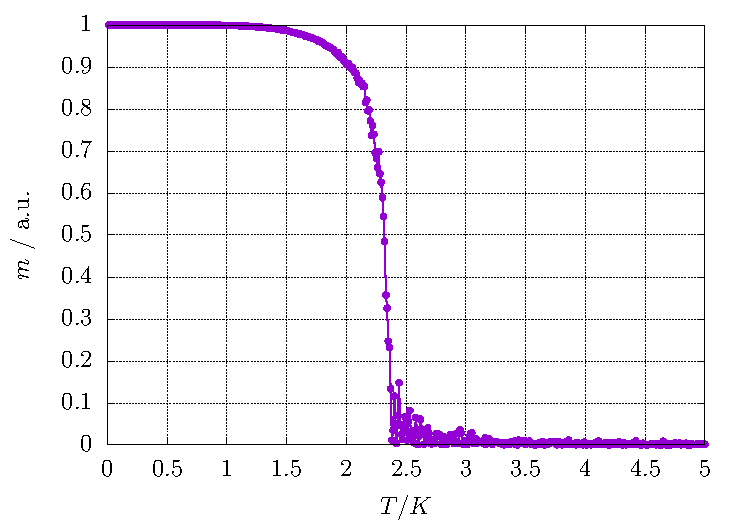
\includegraphics[width=.5\columnwidth]{P4.pdf}
            \caption{$32\times 32$ 格点的 Ising 模型磁化强度关于温度的函数曲线.}
            \label{4-M-T}
        \end{figure}
        \item[3)] 由图 \ref{4-M-T} 中可见,该 Ising 模型的临界温度约 $2.3$ K,利用平均场理论,临界温度的严格解为
        \begin{align}
            \tanh^2\frac{2J}{kT_c}=\frac{1}{2}\Longrightarrow T_c=\frac{2J}{k\ln(1+\sqrt{2})}=\frac{2\times 1}{1\times\ln(1+\sqrt{2})}\text{ K}=2.269\text{ K}.
        \end{align}
        两者符合得较好.
    \end{itemize}
    附 Fortran 代码如下:
    \begin{lstlisting}
program main
    use mpi
    implicit none
    real(8), parameter :: pi = acos(-1.d0), kB = 1.d0
    integer :: ntasks, id, rc
    integer, allocatable :: status(:)
    integer :: i, n, clock
    integer, allocatable :: seed(:)
    real(8) :: r

    real(8) :: T = .01d0, dT = .01d0, T_final = 5.d0, beta
    integer, parameter :: L_x = 32, L_y = 32
    integer :: lattice(0:L_x - 1,0:L_y - 1) = 1
    integer :: x, y
    integer, parameter :: n_warmup = 10000, n_evol = 100000
    real(8) :: J = 1.d0, B = 0.d0
    real(8) :: M, M_sqr, E_tmp, E, E_sqr, M_ave, M_sqr_ave, chi, E_ave, E_sqr_ave, C

    ! initialize MPI environment
    call MPI_INIT(rc)
    call MPI_COMM_SIZE(MPI_COMM_WORLD, ntasks, rc)
    call MPI_COMM_RANK(MPI_COMM_WORLD, id, rc)
    allocate(status(MPI_STATUS_SIZE))

    ! initialize seeds for different processes
    if (id == 0) then
        call SYSTEM_CLOCK(clock)
        call RANDOM_SEED(size = n)
        allocate(seed(n))
        do i = 1, n
            seed(i) = clock + 37 * i
        end do
        call RANDOM_SEED(PUT = seed)
        deallocate(seed)
        do i = 1, ntasks - 1
            call RANDOM_NUMBER(r)
            clock = clock + Int(r * 1000000)
            call MPI_SEND(clock, 1, MPI_INTEGER, i, i, MPI_COMM_WORLD, rc)
        end do
    else
        call MPI_RECV(clock, 1, MPI_INTEGER, 0, id, MPI_COMM_WORLD, status, rc)
        call RANDOM_SEED(size = n)
        allocate(seed(n))
        do i = 1, n
            seed(i) = clock + 37 * i
        end do
        call RANDOM_SEED(PUT = seed)
        deallocate(seed)
    end if

    if (id == 0) then
        open(unit = 1, file = 'data.txt', status = 'unknown')
        write(*,'(4a20)') 'T', 'm', 'chi', 'C'
    end if

    do while (T < T_final)
        beta = 1.d0 / kB / T
        M = 0.d0
        M_sqr = 0.d0
        E = 0.d0
        E_sqr = 0.d0

        ! warm up
        do i = 1, n_warmup
            call EVOLUTION(lattice, L_x, L_y, beta, B, J)
        end do

        ! evolution
        do i = 1, n_evol
            call EVOLUTION(lattice, L_x, L_y, beta, B, J)
            M = M + sum(lattice)
            M_sqr = M_sqr + sum(lattice)**2
            E_tmp = 0.d0
            do x = 0, L_x - 2
                do y = 0, L_y - 2
                    E_tmp = E_tmp + lattice(x, y) * (lattice(x + 1, y) + lattice(x, y + 1))
                end do
            end do
            do x = 0, L_x - 2
                E_tmp = E_tmp + lattice(x, L_y - 1) * (lattice(x + 1, L_y - 1) + lattice(x, 0))
            end do
            do y = 0, L_y - 2
                E_tmp = E_tmp + lattice(L_x - 1, y) * (lattice(L_x - 1, y + 1) + lattice(0, y))
            end do
            E_tmp = E_tmp + lattice(L_x - 1, L_y - 1) * (lattice(0, L_y - 1) + Lattice(L_x - 1, 0))
            E_tmp = - E_tmp * J - B * sum(lattice)
            E = E + E_tmp
            E_sqr = E_sqr + E_tmp**2
        end do
        call MPI_REDUCE(M, M_ave, 1, MPI_REAL8, MPI_SUM, 0, MPI_COMM_WORLD, rc)
        call MPI_REDUCE(M_sqr, M_sqr_ave, 1, MPI_REAL8, MPI_SUM, 0, MPI_COMM_WORLD, rc)
        call MPI_REDUCE(E, E_ave, 1, MPI_REAL8, MPI_SUM, 0, MPI_COMM_WORLD, rc)
        call MPI_REDUCE(E_sqr, E_sqr_ave, 1, MPI_REAL8, MPI_SUM, 0, MPI_COMM_WORLD, rc)
        if (id == 0) then
            M_ave = M_ave / dble(ntasks * n_evol)
            M_sqr_ave = M_sqr_ave / dble(ntasks * n_evol)
            chi = beta * (M_sqr_ave - M_ave**2)
            E_ave = E_ave / dble(ntasks * n_evol)
            E_sqr_ave = E_sqr_ave / dble(ntasks * n_evol)
            C = kB * beta**2 / dble((L_x) * (L_y)) * (E_sqr_ave - E_ave**2)
            write(*,'(4f20.10)') T, M_ave / dble((L_x) * (L_y)), chi, C
            write(1,'(4f20.10)') T, M_ave / dble((L_x) * (L_y)), chi, C
        end if
        T = T + dT
    end do

    if (id == 0) then
        close(1)
    end if

    ! done with MPI
    call MPI_FINALIZE(rc)
end program main

subroutine EVOLUTION(lattice, L_x, L_y, beta, B, J)
    implicit none
    integer, intent(in) :: L_x, L_y
    integer, intent(inout) :: lattice(0:L_x - 1, 0:L_y - 1)
    real(8), intent(in) :: beta, B, J
    real(8) :: r
    integer :: x, y
    real(8) :: dE

    call RANDOM_NUMBER(r)
    x = floor(r * dble(L_x))
    call RANDOM_NUMBER(r)
    y = floor(r * dble(L_y))

    dE = 0.d0
    dE = dE + 2.d0 * J * lattice(x,y) * (lattice(modulo(x - 1, L_x), y)&
        + lattice(modulo(x + 1, L_x), y)&
        + lattice(x, modulo(y - 1, L_y))&
        + lattice(x, modulo(y + 1, L_y)))&
        + 2.d0 * B * dble(lattice(x,y))

    call RANDOM_NUMBER(r)
    if (r < exp(-beta * dE)) then
        lattice(x,y) = -lattice(x,y)
    end if
end subroutine EVOLUTION
    \end{lstlisting}
\end{sol}
\clearpage

\begin{prob}
    弱耦合自旋为零玻色气体的相互作用算符为
    \[
        \Omega=\frac{1}{2V}g\sum_{\vec{p}_1+\vec{p}_2=\vec{p}_1'+\vec{p}_2'}a_{\vec{p}_1'}^{\dagger}a_{\vec{p}_2'}^{\dagger}a_{\vec{p}_2}a_{\vec{p}_1}\quad g>0
    \]
    其中 $a_{\vec{p}}$ 和 $a_{\vec{p}^{\dagger}}$ 为动量表象的湮灭产生算符,$g$ 为耦合常数. 令 $\lvert\{n_{\vec{p}}\}\rangle$ 为自由波色气体的能量本征态,其中 $n_{\vec{p}}$ 为动量 $\vec{p}$ 态的占据数.
    \begin{itemize}
        \item[1)] 证明相互作用能密度的平均值
        \[
            E[\{n_{\vec{p}}\}]\equiv\frac{1}{V}\langle\{n_{\vec{p}}\}\rvert\Omega\lvert\{n_{\vec{p}}\}\rangle=g\rho^2-\frac{g}{2V^2}\sum_{\vec{p}}n_{\vec{p}}^2-\frac{g\rho}{2V}
        \]
        其中 $\rho$ 玻色子的数密度.
        \item[2)] 在热力学极限下比较有 Bose-Einstein 凝聚的上述平均值 $E$ 和没有 Bose-Einstein 凝聚的上述平均值 $E'$,证明
        \[
            E<E'\tag{\text{5 分}}
        \]
    \end{itemize}
\end{prob}
\begin{pf}
    \begin{itemize}
        \item[1)] 自由波色气体的能量本征态为
        \begin{align}
            \lvert\{n_{\vec{p}}\}\rangle=\prod_{\vec{p}}\frac{\left(a_{\vec{p}}^{\dagger}\right)^{n_{\vec{p}}}}{\sqrt{n_{\vec{p}}!}}\lvert 0\rangle.
        \end{align}
        相互作用能密度的平均值为
        {\small
        \begin{align}
            \notag&E[\{n_{\vec{p}}\}]=\frac{1}{V}\langle\{n_{\vec{p}}\}\rvert\Omega\lvert\{n_{\vec{p}}\}\rangle\\
            \notag=&\frac{g}{V^2}\prod_{\vec{p},\vec{p}'}\sum_{\vec{p}_1+\vec{p}_2=\vec{p}_1'+\vec{p}_2'}\frac{1}{\sqrt{n_{\vec{p}'}!}}\frac{1}{\sqrt{n_{\vec{p}}!}}\langle 0\rvert \left(a_{\vec{p}'}\right)^{n_{\vec{p}}}a_{\vec{p}_1'}^{\dagger}a_{\vec{p}_2'}^{\dagger}a_{\vec{p}_2}a_{\vec{p}_1}\left(a_{\vec{p}}^{\dagger}\right)^{n_{\vec{p}}}\lvert 0\rangle\\
            \notag=&\frac{g}{V^2}\prod_{\vec{p},\vec{p}'}\sum_{\vec{p}_1+\vec{p}_2=\vec{p}_1'+\vec{p}_2'}\frac{1}{\sqrt{n_{\vec{p}'}!}}\frac{1}{\sqrt{n_{\vec{p}}!}}\langle 0\rvert \left(a_{\vec{p}'}\right)^{n_{\vec{p}}}a_{\vec{p}_1'}^{\dagger}a_{\vec{p}_2'}^{\dagger}a_{\vec{p}_2}\left\{[a_{\vec{p}_1},a_{\vec{p}}^{\dagger}]+a_{\vec{p}}^{\dagger}a_{\vec{p}_1}\right\}\left(a_{\vec{p}}^{\dagger}\right)^{n_{\vec{p}}-1}\lvert 0\rangle\\
            \notag=&\frac{g}{V^2}\prod_{\vec{p},\vec{p}'}\sum_{\vec{p}_1+\vec{p}_2=\vec{p}_1'+\vec{p}_2'}\frac{1}{\sqrt{n_{\vec{p}'}!}}\frac{1}{\sqrt{n_{\vec{p}}!}}\langle 0\rvert \left(a_{\vec{p}'}\right)^{n_{\vec{p}}}a_{\vec{p}_1'}^{\dagger}a_{\vec{p}_2'}^{\dagger}a_{\vec{p}_2}\left\{\delta_{\vec{p}_1\vec{p}}+a_{\vec{p}}^{\dagger}a_{\vec{p}_1}\right\}\left(a_{\vec{p}}^{\dagger}\right)^{n_{\vec{p}}-1}\lvert 0\rangle\\
            \notag=&\frac{g}{V^2}\prod_{\vec{p},\vec{p}'}\sum_{\vec{p}_1+\vec{p}_2=\vec{p}_1'+\vec{p}_2'}\frac{1}{\sqrt{n_{\vec{p}'}!}}\frac{1}{\sqrt{n_{\vec{p}}!}}\langle 0\rvert \left(a_{\vec{p}'}\right)^{n_{\vec{p}}}a_{\vec{p}_1'}^{\dagger}a_{\vec{p}_2'}^{\dagger}a_{\vec{p}_2}\left\{\delta_{\vec{p}_1\vec{p}}+a_{\vec{p}}^{\dagger}\delta_{\vec{p}_1\vec{p}}+\left(a_{\vec{p}}^{\dagger}\right)^2a_{\vec{p}_1}\right\}\left(a_{\vec{p}}^{\dagger}\right)^{n_{\vec{p}}-2}\lvert 0\rangle\\
            \notag&\cdots\\
            \notag=&\frac{g}{V^2}\prod_{\vec{p},\vec{p}'}\sum_{\vec{p}_1+\vec{p}_2=\vec{p}_1'+\vec{p}_2'}\frac{1}{\sqrt{n_{\vec{p}'}!}}\frac{1}{\sqrt{n_{\vec{p}}!}}\langle 0\rvert \left(a_{\vec{p}'}\right)^{n_{\vec{p}}}a_{\vec{p}_1'}^{\dagger}a_{\vec{p}_2'}^{\dagger}a_{\vec{p}_2}\left\{\delta_{\vec{p}_1\vec{p}}\sum_{n=0}^{n_{\vec{p}}-1}\left(a_{\vec{p}}^{\dagger}\right)^n+\left(a_{\vec{p}}^{\dagger}\right)^{n_{\vec{p}}}a_{\vec{p}_1}\right\}\lvert 0\rangle\\
            \notag=&\frac{g}{V^2}\prod_{\vec{p},\vec{p}'}\sum_{\vec{p}_1,\vec{p}_2,\vec{p}_1',\vec{p}_2'=\vec{p}_1+\vec{p}_2-\vec{p}_1'}\frac{1}{\sqrt{n_{\vec{p}'}!}}\frac{1}{\sqrt{n_{\vec{p}}!}}\langle 0\rvert \left(a_{\vec{p}'}\right)^{n_{\vec{p}}}a_{\vec{p}_1'}^{\dagger}a_{\vec{p}_2'}^{\dagger}a_{\vec{p}_2}\left\{\delta_{\vec{p}_1\vec{p}}\sum_{n=0}^{n_{\vec{p}}-1}\left(a_{\vec{p}}^{\dagger}\right)^n+\left(a_{\vec{p}}^{\dagger}\right)^{n_{\vec{p}}}a_{\vec{p}_1}\right\}\lvert 0\rangle\\
            \notag=&\frac{g}{V^2}\prod_{\vec{p},\vec{p}'}\sum_{\vec{p}_2,\vec{p}_1',\vec{p}_2'=\vec{p}+\vec{p}_2-\vec{p}_1'}\frac{1}{\sqrt{n_{\vec{p}'}!}}\frac{1}{\sqrt{n_{\vec{p}}!}}\langle 0\rvert \left(a_{\vec{p}'}\right)^{n_{\vec{p}}}a_{\vec{p}_1'}^{\dagger}a_{\vec{p}_2'}^{\dagger}a_{\vec{p}_2}\left\{\sum_{n=0}^{n_{\vec{p}}-1}\left(a_{\vec{p}}^{\dagger}\right)^n\right\}\lvert 0\rangle\\
            \notag=&\frac{g}{V^2}\prod_{\vec{p},\vec{p}'}\sum_{\vec{p}_1',\vec{p}_2'=2\vec{p}-\vec{p}_1'}\frac{1}{\sqrt{n_{\vec{p}'}!}}\frac{1}{\sqrt{n_{\vec{p}}!}}\langle 0\rvert \left(a_{\vec{p}'}\right)^{n_{\vec{p}}}a_{\vec{p}_1'}^{\dagger}a_{\vec{p}_2'}^{\dagger}\left\{\sum_{n=0}^{n_{\vec{p}}-1}\sum_{m=0}^{n-1}\left(a_{\vec{p}}^{\dagger}\right)^m\right\}\lvert 0\rangle\\
            \notag=&\frac{g}{V^2}\prod_{\vec{p},\vec{p}'}\frac{1}{\sqrt{n_{\vec{p}'}!}}\frac{1}{\sqrt{n_{\vec{p}}!}}\langle 0\rvert\left\{\sum_{l=0}^{n_{\vec{p}'-1}}\left(a_{\vec{p}'}\right)^l\right\}a_{2\vec{p}-\vec{p}'}^{\dagger}\left\{\sum_{n=0}^{n_{\vec{p}}-1}\sum_{m=0}^{n-1}\left(a_{\vec{p}}^{\dagger}\right)^m\right\}\lvert 0\rangle\\
            \notag=&\frac{g}{V^2}\prod_{\vec{p},\vec{p}'}\frac{1}{\sqrt{n_{\vec{p}'}!}}\frac{1}{\sqrt{n_{\vec{p}}!}}\langle 0\rvert\left\{\sum_{l=0}^{n_{\vec{p}-1}}\sum_{k=0}^{l-1}\left(a_{\vec{p}'}\right)^k\delta_{\vec{p}',2\vec{p}-\vec{p}'}\right\}\left\{\sum_{n=0}^{n_{\vec{p}}-1}\sum_{m=0}^{n-1}\left(a_{\vec{p}}^{\dagger}\right)^m\right\}\lvert 0\rangle\\
            \notag=&\frac{g}{V^2}\prod_{\vec{p},\vec{p}'}\frac{1}{\sqrt{n_{\vec{p}'}!}}\frac{1}{\sqrt{n_{\vec{p}}!}}\langle 0\rvert\left\{\sum_{l=0}^{n_{\vec{p}-1}}\sum_{k=0}^{l-1}\left(a_{\vec{p}'}\right)^k\delta_{\vec{p},\vec{p}'}\right\}\left\{\sum_{n=0}^{n_{\vec{p}}-1}\sum_{m=0}^{n-1}\left(a_{\vec{p}}^{\dagger}\right)^m\right\}\lvert 0\rangle\\
            \notag=&\frac{g}{V^2}\prod_{\vec{p},\vec{p}'}\frac{1}{\sqrt{n_{\vec{p}'}!}}\frac{1}{\sqrt{n_{\vec{p}}!}}\langle 0\rvert\left\{\sum_{l=0}^{n_{\vec{p}'-1}}(n_{\vec{p}'}-l-1)\left(a_{\vec{p}'}\right)^l\delta_{\vec{p},\vec{p}'}\right\}\left\{\sum_{n=0}^{n_{\vec{p}}-1}(n_{\vec{p}}-n-1)\left(a_{\vec{p}}^{\dagger}\right)^n\right\}\lvert 0\rangle\\
            =&g\rho^2-\frac{g}{2V^2}\sum_{\vec{p}}n_{\vec{p}}^2-\frac{g\rho}{2V}.
        \end{align}
        }
    \end{itemize}
\end{pf}
\end{document}